% !TeX spellcheck = de_DE

%  ******************************************************************************
%  * @file      tex/Modultest                                                   *
%  * @author    Mario Hesse                                                     *
%  * @version   v0.1.1                                                          *
%  * @date      16.10.2019                                                      *
%  ******************************************************************************

\section{Modultest/Messungen}

In diesem Abschnitt werden im Zuge der Arbeit erstellte Module getestet und Messungen dokumentiert. Mit dem Paket Tikz und PGF Plots kann man Daten direkt in Latex aufbereiten. Diagramme können in der \emph{tikzpicture} Umgebung erstellt werden. Typischerweise werden Diagramme in eine \emph{figure} Umgebung eingebettet, damit man sie wie gewöhnliche Abbildung behandeln kann.

\begin{figure}[htbp]
	\centering
	
	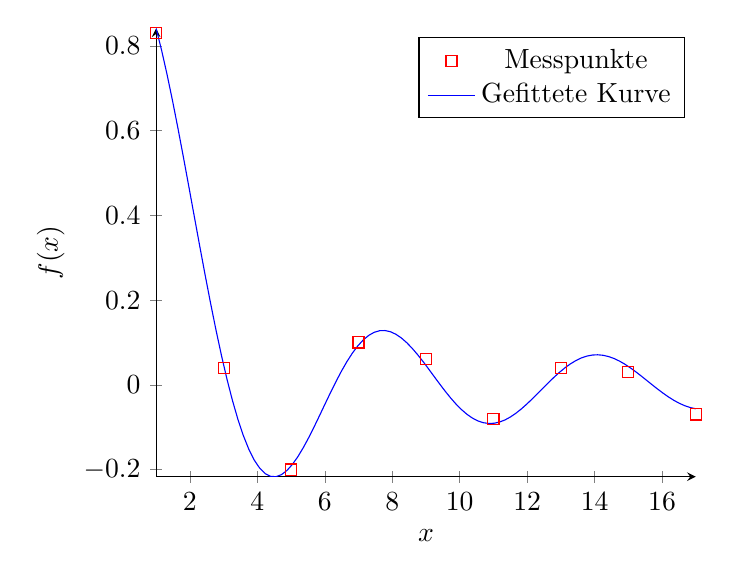
\begin{tikzpicture} 					% Begin einer neuen Grafik
		\begin{axis}[							% Begin des Achsen- bzw. Plotbereichs
		axis lines = left,						% Die Achsen des Plots sind rechts und unten			
		xlabel = $x$,							% Beschriftung der X-Achse
		ylabel = {$f(x)$},						% Beschriftung der Y-Achse
		]
		
		\addplot[								% Definition 1. Plot
		color=red,								% Linienfarbe ist Rot
		mark=square,							% Marker werden als Kästchen gezeichnet
		only marks,								% Es sollen nur Marken ohne Linie angezeigt werden
		]
		coordinates {							% Datenpunkte (x, y)
			(1, 0.83)
			(3, 0.04)
			(5, -0.20)
			(7, 0.10)
			(9, 0.06)
			(11,-0.08)
			(13,0.04)
			(15,0.03)
			(17,-0.07)
		};
		\addlegendentry{Messpunkte}					% Eintrag wird zur Legende hinzugefügt
		
		
		\addplot [								% Definition 2. Plot
		domain=1:17, 								% X-Bereich in dem geplottet werden soll
		samples=100, 								% Anzahl an Einzelpunkten, die für den Plot berechnet werden
		color=blue,									% Linienfarbe ist blau
		]
		{sin(deg(x))/x};							% Zu plottende Funktion
		\addlegendentry{Gefittete Kurve}			% Eintrag wird zu Legende hinzugefügt
		
		\end{axis}							% Ende des Achsen- bzw. Plotbereichs
	\end{tikzpicture}
	
	\caption{Ein in Latex gerendertes Diagramm}
	\label{pic:LatexDiagramm}
\end{figure}


